\documentclass[]{report}
\usepackage{amsmath,amsfonts,graphicx}
%\usepackage{multirow}
%\usepackage{pslatex}
%\usepackage{tabularx}
%\usepackage{comment}
%\usepackage{xspace}
%\usepackage{array}

%\usepackage{hyperref}

%\usepackage{caption}
%\DeclareCaptionFont{white}{\color{white}}
%\DeclareCaptionFormat{listing}{\colorbox{gray}{\parbox{\textwidth}{#1#2#3}}}

\def\species{\mathrm{sp}}
\def\phase{\mathrm{ph}}
\def\massfrac{\chi}
\def\flux{\mathbf{F}}
\def\darcyvel{\mathbf{v}}
\def\energydens{\mathcal{E}}
\def\d{\mathrm{d}}

\newcommand{\uo}{\mbox{UO\textsubscript{2}}\xspace}

\setcounter{secnumdepth}{3}


\begin{document}


\title{Buckley-Leverett Tests}
\author{CSIRO}
\maketitle

\tableofcontents

\chapter{Single Phase}


MOOSE is compared with a simple single-phase one-dimensional
Buckley-Leverett problem\footnote{SE Buckley and MC Leverett (1942)
  ``Mechanism of fluid displacements in sands''.  Transactions of the
  AIME {\bf 146} 107--116}.  The single-phase fluid moves in a region
$0\leq x\leq 15$\,m.  A fully-saturated front initially sits at
position $x=5$, while the region $x>5$ is initially unsaturated.  With
zero suction function $P_{c} = 0$, there is no diffusion of the sharp
front, and it progresses towards the right (increasing $x$).  This is
a difficult problem to simulate numerically as maintaining the sharp
front is hard.  The front's speed is independent of the relative
permeability, since the fluid is flowing from a fully-saturated region
(where $\kappa_{\mathrm{rel}}=1$).  This problem is therefore a good
test of the upwinding.

In the simulation below, the pressure at the left boundary is kept
fixed at $P_{0}=0.98$\,MPa, while the right boundary is kept fixed at
$P_{15}=-20000$\,Pa, so the difference is 1\,MPa.  The medium's
permeability is set to $\kappa = 10^{-10}\,\mathrm{m}^{2}$ and its
porosity is $\phi = 0.15$.  It is not possible to use a zero suction
function in the MOOSE implementation, but using the van Genuchten
parameters $\alpha = 10^{-3}$\,Pa$^{-1}$ and $m=0.8$ approximates it.
The fluid viscosity is $\mu = 10^{-3}$\,Pa.s.

The initial condition is
\begin{equation}
P(t=0) = \left\{
\begin{array}{ll}
P_{0} - (P_{0}-P_{15})x/5 & \ \ \ \mbox{for }\ \ x<5 \\
P_{15} & \ \ \ \mbox{for }\ \ x\geq 5
\end{array}
\right. \ ,
\end{equation}
which is shown in
Figure~\ref{bl_setup.figa}.  With the suction function defined above
this gives
\begin{equation}
S(t=0) = \left\{
\begin{array}{ll}
1 & \ \ \ \mbox{for }\ \ x\leq 4.9 \\
0.061 & \ \ \ \mbox{for} \ \ x \geq 5
\end{array}
\right.
\end{equation}

\begin{figure}[htb]
\begin{center}
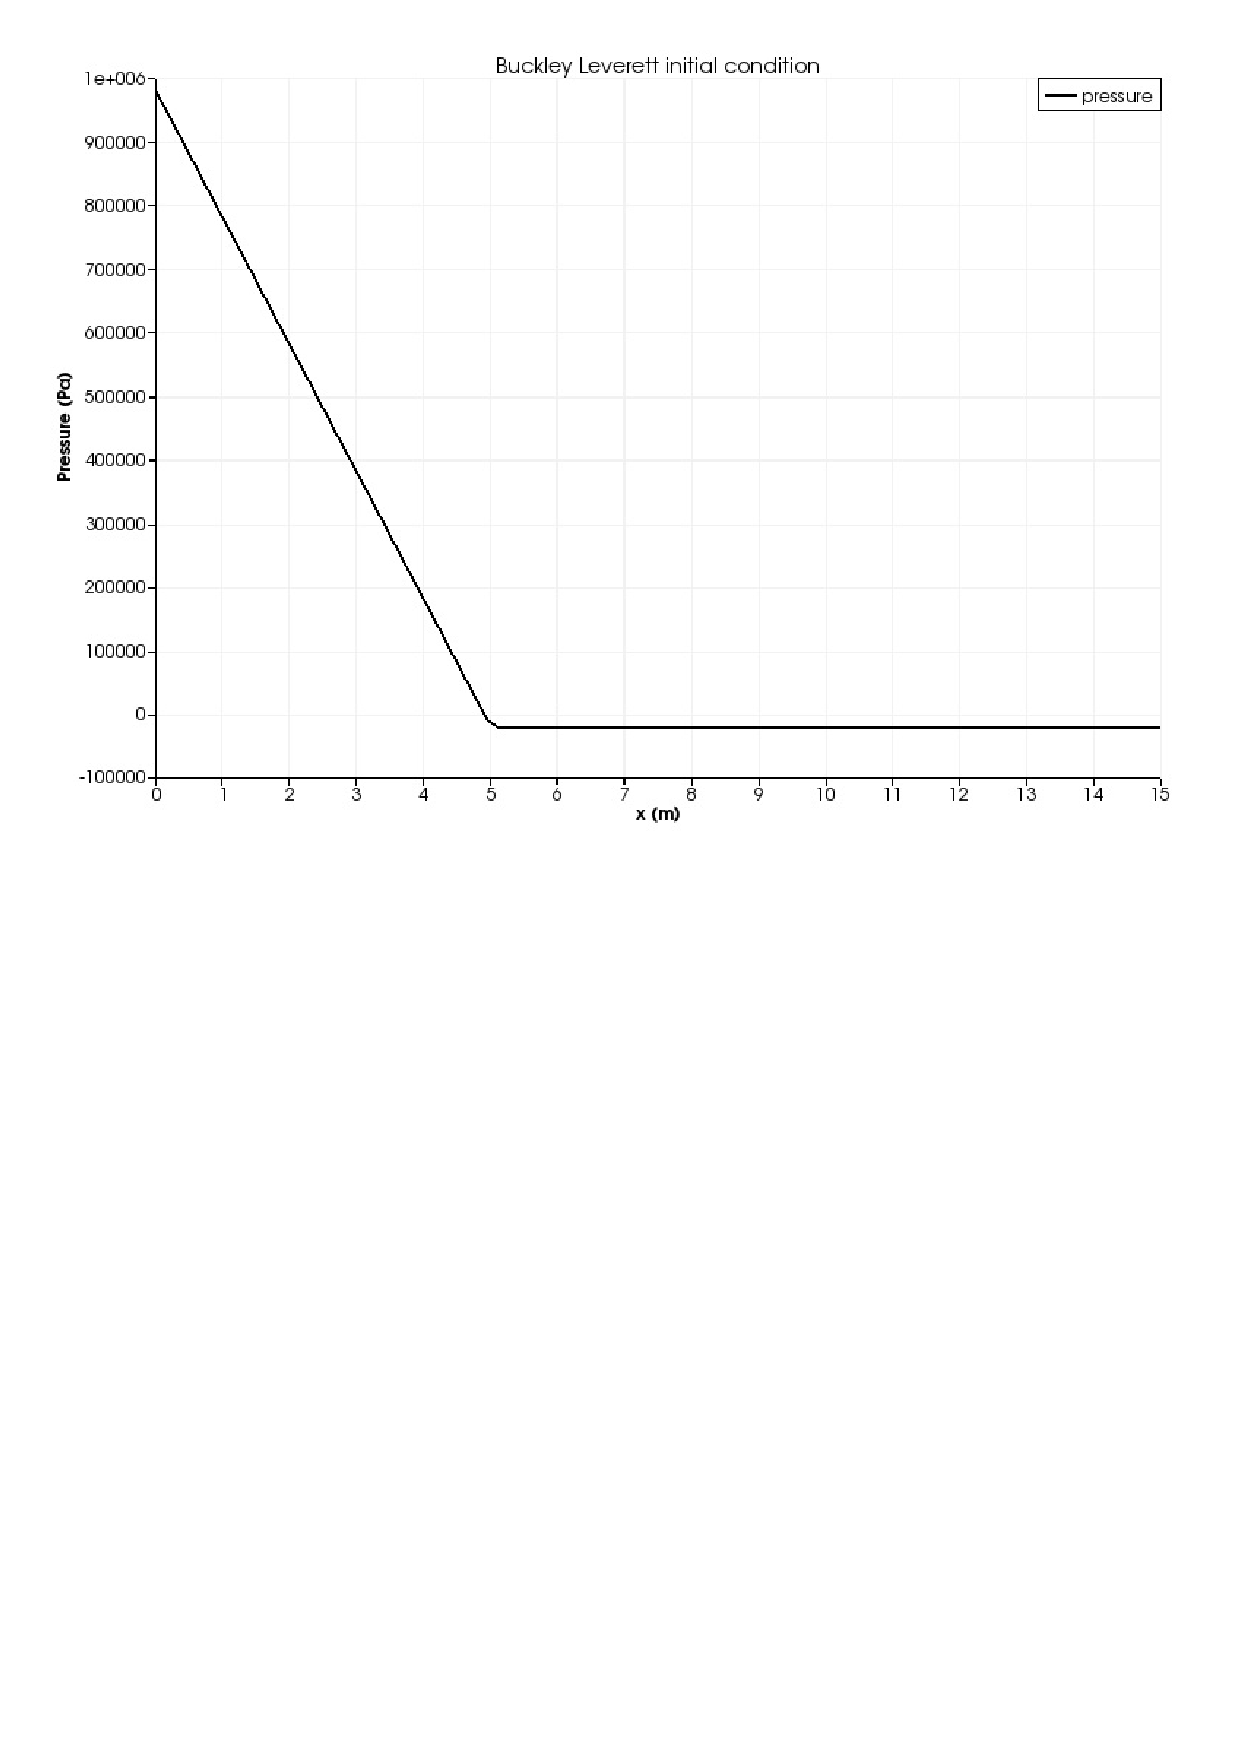
\includegraphics[width=12cm]{bl_initial1.pdf}
\caption{Initial setup of the Buckley-Leverett problem where
  porepressure is a piecewise linear function.  The region
$x\leq 4.9$ is fully saturated, while the region $x>5$ has saturation
  0.061.  During simulation the value $P(x=0)=0.98\times 10^{6}$\,MPa
  is held fixed.}
\label{bl_setup.figa}
\end{center}
\end{figure}

Good approximations for the pressure $P(x,t)$
and the front position $f(t)$ may be determined from
\begin{eqnarray}
\frac{{\mathrm d} f}{{\mathrm d} t} & = & -\frac{\kappa}{\phi\mu}
\left.\frac{\partial  P}{\partial x}\right|_{x = f} \ , \nonumber \\
P(x,t) & = & \left\{
\begin{array}{ll}
P_{0} - (P_{0}-P_{15})x/f & \mbox{ for } x\leq f  \\
P_{15} & \mbox{ for } x>f
\end{array}
\right. \ ,
\label{eqn.predicted.bl.posn.eqna}
\end{eqnarray}
which has solution
\begin{equation}
f(t) = \sqrt{f(0)^{2} + \frac{2\kappa}{\phi\mu}(P_{0}-P_{15})t} \ .
\end{equation}
For the parameters listed above, the front will be at position
$f=9.6$\,m at $t=50$\,s.  This solution is only valid for zero
capillary suction.  A nonzero suction function will tend to diffuse
the sharp front.

With coarse meshes it is impossible to simulate a sharp front, of
course, since the front is spread over at least one element.

Figure~\ref{satfront.figa} shows the results from a MOOSE simulation
with a uniform mesh of size 0.1\,m.  At $t=50$\,s the front in this
simulation sits at $x=9.6$\,m as desired.  However, the simulation
takes 10\,seconds to complete due to the very low values of saturation
obtained for van Genuchten $\alpha=10^{-3}$\,Pa$^{-1}$.  Other
simulations give similar results but run much faster.  For instance,
the test suite uses the van-Genuchten parameter
$\alpha=10^{-4}$\,Pa$^{-1}$, but the front diffuses a little into the
unsaturated region (the front sits between $x=9.7$\,m and $x=10.4$\,m
at $t=50$\,s).

\begin{figure}[htb]
\begin{center}
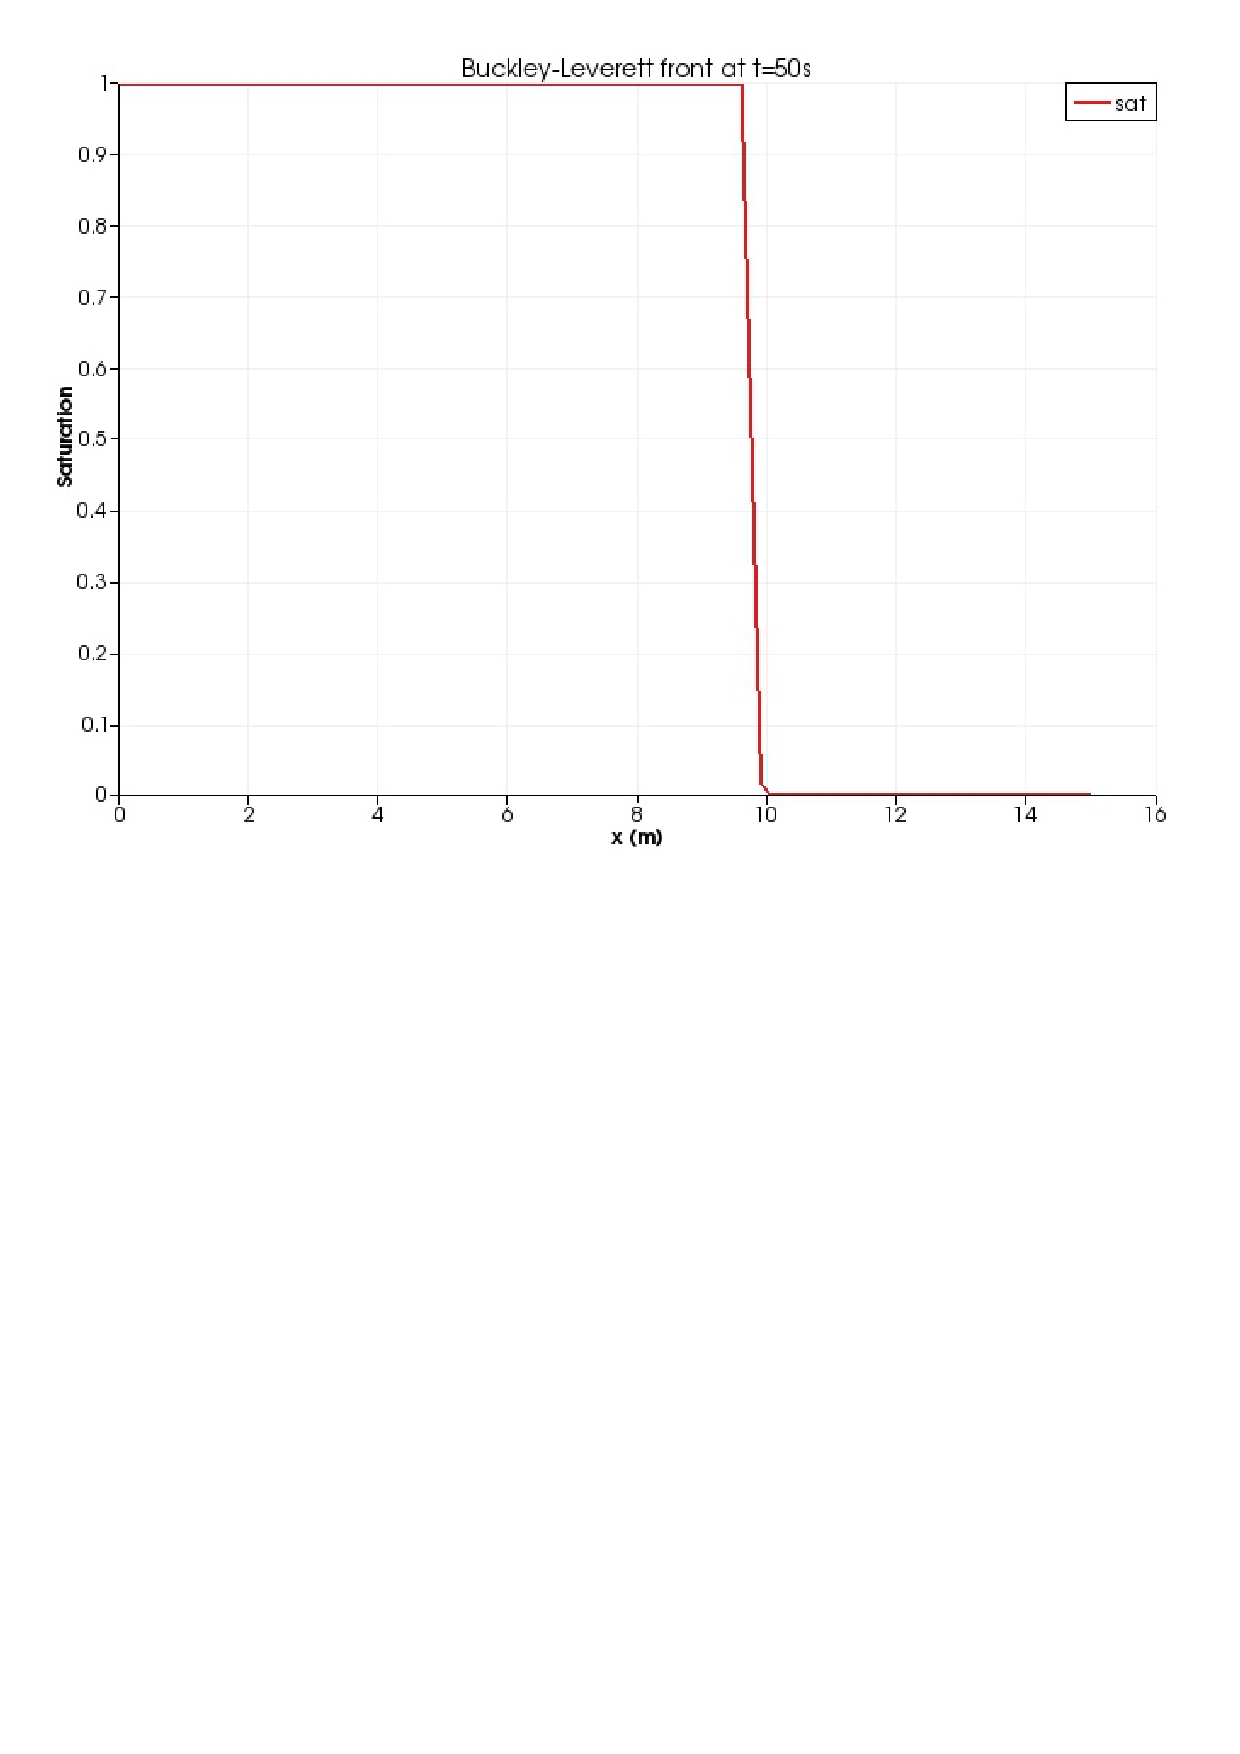
\includegraphics[width=10cm]{bl01_sat1.pdf} \\
$\mbox{}$
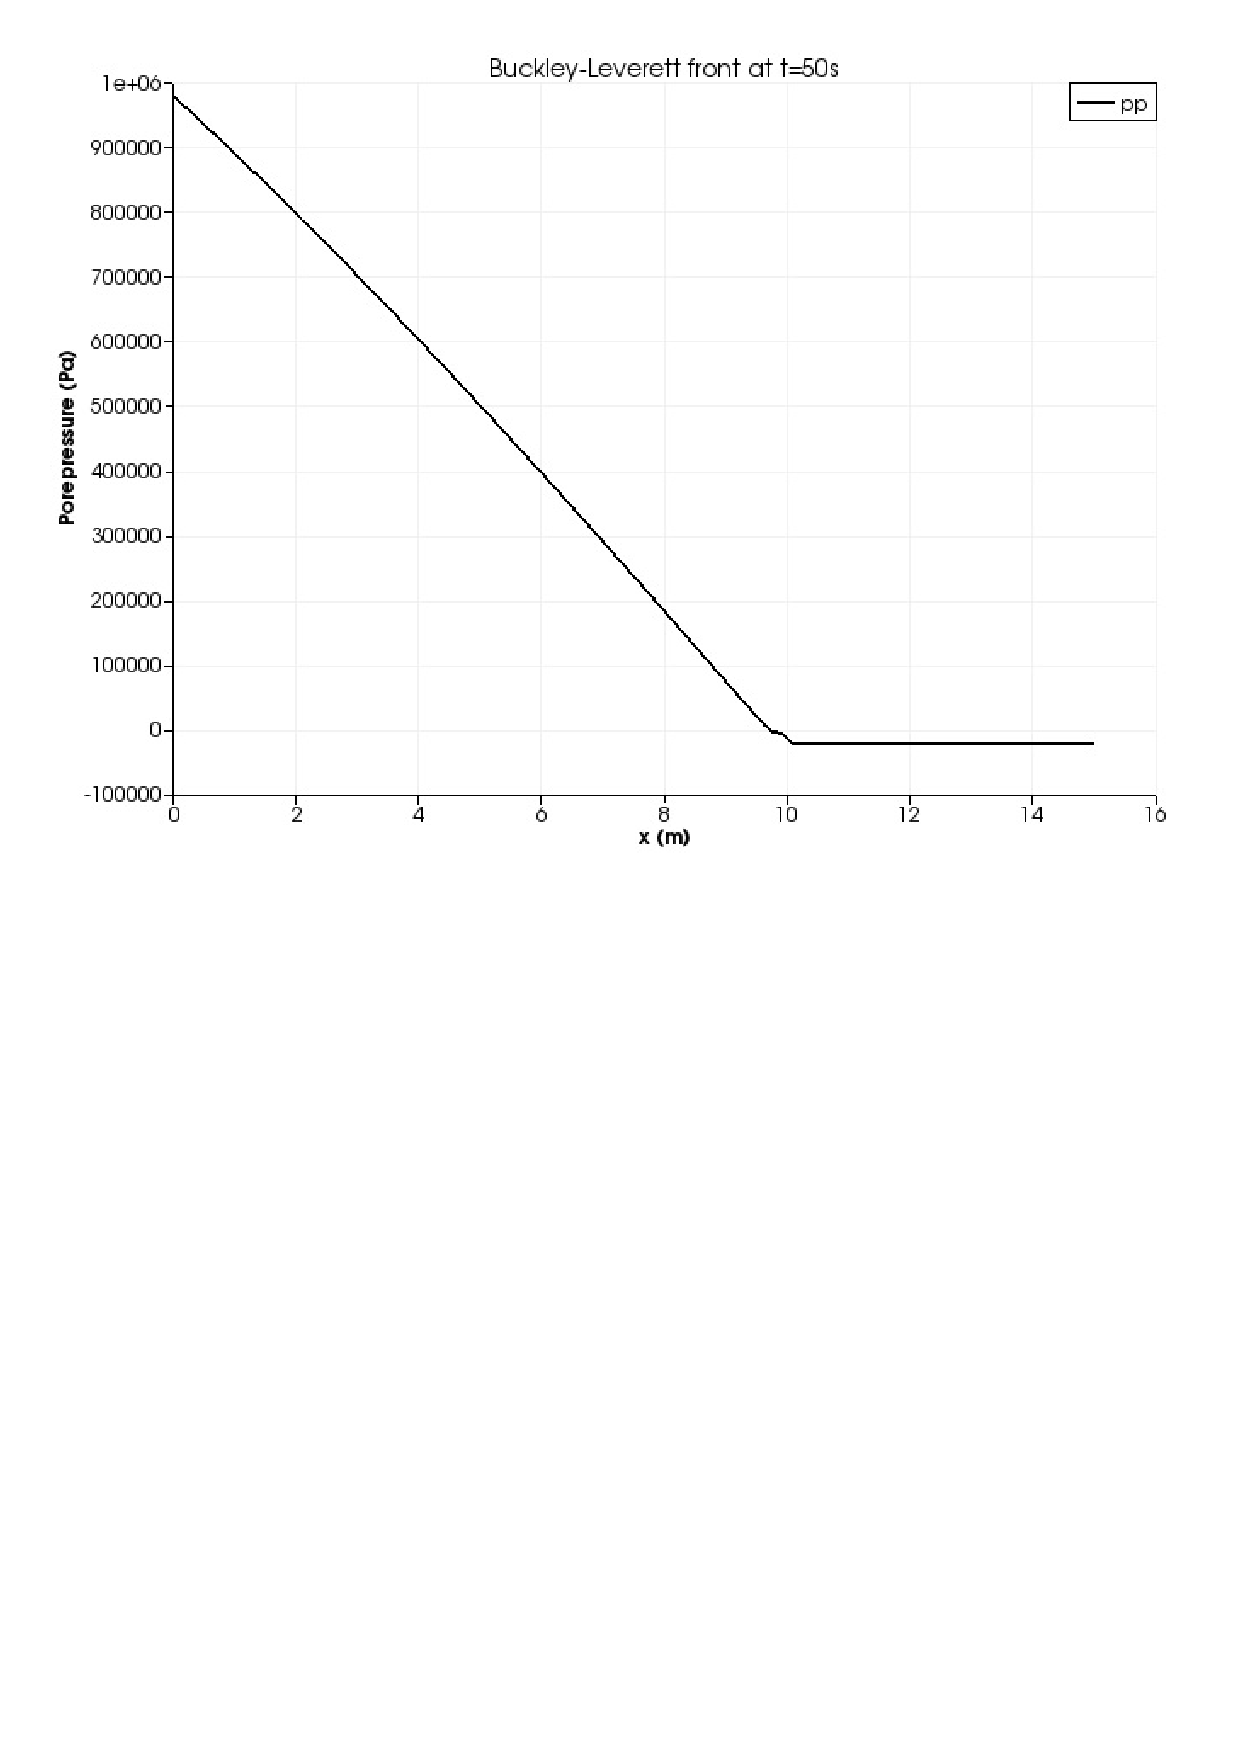
\includegraphics[width=10cm]{bl01_pp1.pdf} \\
\caption{The MOOSE solution of the Buckley-Leverett problem at
  $t=50$\,s.  Top: saturation.  Bottom: porepressure.  The front sits
  between $x=9.6$\,m as expected from the analytical solution.}
\label{satfront.figa}
\end{center}
\end{figure}

\end{document}




